\clearpage{\pagestyle{empty}\cleardoublepage}
\chapter{Integrazione con DLX}

In questo capitolo saranno descritte le problematiche affrontate durante l'integrazione del componente cache all'interno del progetto del DLX gi\`a esistente.

\section{Modifiche al Memory\_stage}

Nella realizzazione del componente si \`e supposto che gli accessi alla cache avvengano in un unico ciclo di clock, cos� facendo si \`e potuto evitare di modificare la pipiline del DLX per inserire degli stalli ogni qualvolta si trovasse nello stadio di memory una  operzione di load o una di store. Le modifiche da apportare al dlx si sono rivelate in questa maniera pi\`u esigue e si sono concentrate nel solo stadio di memory essendo la nostra una cache dati.

In particolare sono stati aggiunti al componente \texttt{Memory\_Stage} i seguenti segnali:\\

\lstset{language=VHDL,  caption=Segnali aggiunti allo stadio di Memory, breaklines=true, basicstyle=\small, showspaces=false, showtabs=false, stringstyle=\ttfamily, showstringspaces=false,  tabsize=3} % basicstyle=\tiny\ttfamily}
\begin{lstlisting}
ready: in std_logic;
memrd: out std_logic;
memwr: out std_logic;
memory_data_register: in std_logic_vector(PARALLELISM-1 downto 0);
load_memory_data_register: in std_logic_vector(PARALLELISM-1 downto 0);
memory_address_register: out std_logic_vector(PARALLELISM-1 downto 0);
\end{lstlisting}


mentre il segnale \texttt{memory\_data\_register} \`e stato sostituito da:\\

\texttt{store\_memory\_data\_register: out std\_logic\_vector(PARALLELISM-1 downto 0);}\\

\`E stata inoltre eliminata la variabile Ram.\\

Le immagini seguenti mostrano come \`e stato modificato lo schema del DLX in seguito all'integrazione della Cache.\\

\begin{figure}[h!]
\centering
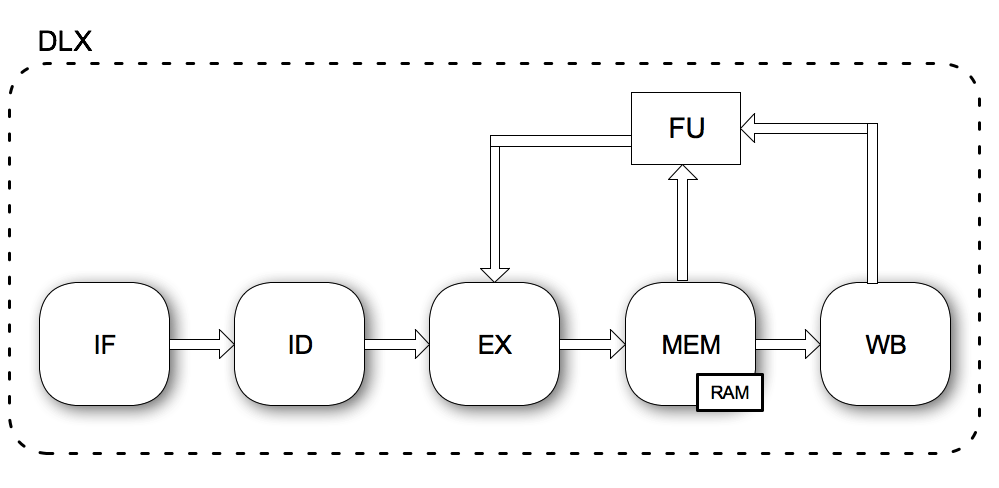
\includegraphics[width=\textwidth]{img/DLX/old_dlx.png}
\caption{Schema della pipeline del DLX originale}
\label{fig:dlx_p1}
\end{figure}

\begin{figure}[h!]
\centering
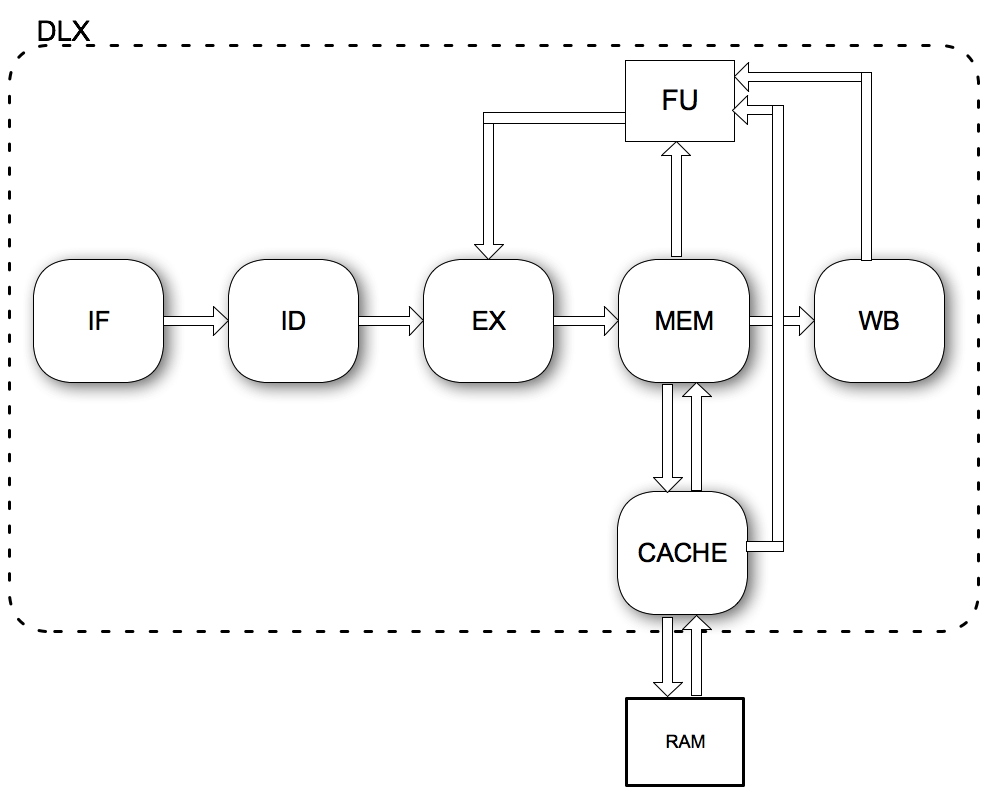
\includegraphics[width=\textwidth]{img/DLX/new_dlx.png}
\caption{Schema della pipeline del DLX con cache integrata}
\label{fig:dlx_p2}
\end{figure}



\newpage
\section{Connessione del componente}

I segnali \texttt{store\_memory\_data\_register} e \texttt{load\_memory\_data\_register} sono connessi rispettivamente al \texttt{ch\_bdata\_in} e al \texttt{ch\_bdata\_out} della cache mentre il \texttt{memory\_data\_register} \`e collegato al bus indirizzi della cache (\texttt{ch\_baddr}).\\
Il segnale ready (connesso al \texttt{ch\_ready} della cache) viene asserito alla fine di ogni ciclo di lettura e scrittura ed indica al processore che il dato proveniente dalla cache � disponibile per la lettura o che la scrittura \`e terminata e pu\`o avere luogo un nuovo ciclo di bus.\\
I rimanenti due segnali \texttt{memrd} e \texttt{memwr} sono rispettivamente collegati ai segnail della cache \texttt{ch\_memrd} e \texttt{ch\_memwr}.\\
A livello di codice nel processo async sono stati modificati i rami del "case a\_opcode\_high is" inerenti la load e la store.\\

\subsection{Istruzione load}

Nel caso di un'istruzione load, il codice \`e stato modificato come illustrato di seguito:\\

\lstset{language=VHDL, caption=Codice dell'istruzione load, breaklines=true, basicstyle=\small, showspaces=false, showtabs=false, stringstyle=\ttfamily, showstringspaces=false,  tabsize=3} % basicstyle=\tiny\ttfamily}

\begin{lstlisting}
memory_address_register <= alu_exit_buffer;
memrd <= '1';	
wait until ready = '1' and ready'event;
memrd <= '0' after TIME_UNIT/3;
dest_register <= a_rd_i;
dest_register_data <= load_memory_data_register;
data_out <= load_memory_data_register;	
\end{lstlisting}


L'uscita dell'ALU viene inviata al bus indirizzi e viene attivato il segnale \texttt{memrd} che sveglia il processo \texttt{cache\_dlx\_process} della cache, dopodich\`e l'istruzione wait until pone il processo in attesa di un fronte del segnale ready.\\
Appena il ready viene attivato il dato proveniente dalla cache viene inviato alla barriera dei registri dello stadio di Write-Back. Infine il segnale \texttt{memrd} viene riportato a 0, ma con un ritardo di TIME\_UNIT/3 necessario per poter rendere visibile l'impulso del segnale in fase di simulazione.\\

L'utilizzo dell'istruzione wait until si \`e reso necessario in alternativa alla realizzazione di un processo separato che sul fronte del ready effettuasse la scrittura dei dati provenienti dal bus sui registri di uscita, in quanto con quest'ultima soluzione si avrebbero due processi distinti in grado di modificare i valori dei segnali \texttt{data\_out} e \texttt{dest\_register\_data} cosa che d\`a luogo a dei conflitti in fase di simulazione.\\
Impiegare la wait until ha comportato come unico effetto collaterale lo spostamento dei segnali presenti nella sesitivity list del processo async nella lista dei parametri della wait on posta come prima istruzione del processo.\\

\subsection{Istruzione store}

La strutture della store risulta simile a quella della load:

\lstset{language=VHDL, caption=Codice dell'istruzione store,  breaklines=true, basicstyle=\small, showspaces=false, showtabs=false, stringstyle=\ttfamily, showstringspaces=false,  tabsize=3} % basicstyle=\tiny\ttfamily}

\begin{lstlisting}
store_memory_data_register <= memory_data_register_buffer; 
memory_address_register <= alu_exit_buffer;
memwr <= '1';
wait until ready = '1' and ready'event;
memwr <= '0' after TIME_UNIT/3;
\end{lstlisting}

In questo caso oltre all'indirizzo viene mandato sul bus dati verso la cache il dato da memorizzare e viene attivato il \texttt{memwr}. \\
Come in precedenza anche qui il processo attende il fronte del ready e riporta a zero \texttt{memwr} con un ritardo di TIME\_UNIT/3.


